Remappings can be either logical or materialized.

The former are created by joining any table with a remapping table, producing the results in the query output.
In the latter case, on the other hand, the results are physically stored on the data warehouse and do not require any join operation.

Let's now analyze the advantages and disadvantages of each remapping technique.

\subsubsection{Query performance}
    The type of remapping chosen can directly influence the performance of a query.

    \paragraph{Logical remappings}
        Logical remappings require to join each value of a given table with the remapping.
        This operation is applied to a large amount queries used by Axpo, since they require some information in a specific notation.
        
        The cost of the join is however low, since these remapping tables are usually very small, ranging from tens to a couple hundred rows.
        As such a single join can be computed very quickly, but it can become a problem if these operations need to be applied for almost each query.
        
    \paragraph{Materialized remappings}
        Materialized remappings require no additional overhead, since the remapped information are physically stored along the other data.
        
        This choice is ideal for values which are always used in their remapped notation.
        For example, each provider uses its own hour notation, while all Axpo tools use a standard numeric notation ranging from 1 to 25.
        
        Instead of having to perform a join for \textunderscore{every} query, it is more efficient to memorized this value directly into the table, removing the join overhead.
    
    
\subsubsection{Query complexity}
    Queries become more complex since they require join operations with additional tables.
    This scenario is even more complex when multiple remappings are needed for the same table.
    
    \paragraph{Logical remappings}
        For local remappings, each remapping needed results in a join operation.
        
        Sometimes, multiple columns referring to the same type of information need to be remapped.
        This leads to a more complex query, in which it is necessary to remember the name of each remap in order to avoid confusion.
        
        \begin{figure}
            \centering
            \begin{subfigure}{\textwidth}
                \centering
                \fbox{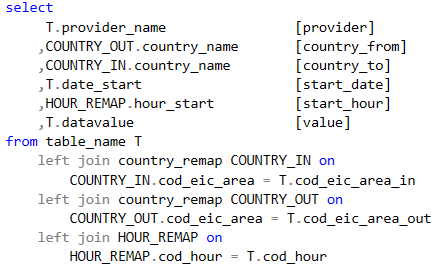
\includegraphics[width=.5\textwidth]{res/dwh/remap_logical.png}}
                \subcaption{Logical}
                \label{fig:dwh:remapping:complexity:logical}
            \end{subfigure}
            
            \begin{subfigure}{\textwidth}
                \centering
                \fbox{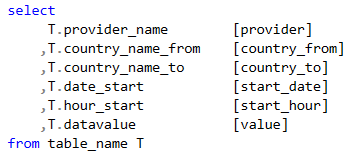
\includegraphics[width=.4\textwidth]{res/dwh/remap_materialized.png}}
                \subcaption{Materialized}
                \label{fig:dwh:remapping:complexity:materialized}
            \end{subfigure}
            
            \caption{Query complexity for different remappings. Both queries produce the same output.}
            \label{fig:dwh:remapping:complexity}
        \end{figure}
        
        As an example, the query shown in Figure \ref{fig:dwh:remapping:complexity:logical} represents a query using logical remappings.
        As we can see, multiple join operations are needed, making the query harder to read.
        
    \paragraph{Materialized remappings}
        Materialized remappings do not need any join operation, since the data is directly present in the table.
        As a consequence, queries are both easier to write and to read.
    
        The query shown in Figure \ref{fig:dwh:remapping:complexity:materialized} represents the same query as above, but uses materialized remappings.
        The query is certainly easier to read and to understand, and the possibility of making errors is minimized.

\subsubsection{Data insertion}
    When a new row is inserted additional operations have to be performed depending on the remapping type.
    
    \paragraph{Logical remappings}
        Logical remappings are more convenient during insertion, since they do not require any additional operation on the values inserted.
        
        The only check needed is that each value to be remapped is present in the remapping table.
        
        Otherwise an alert must be raised and an appropriate remapping has to be created.
    
    \paragraph{Materialized remappings}
        In case of materialized remappings, it is necessary to compute each remapping prior to the insertion operation.
        
        In case of missing values, there are two possibilities: either the row is not inserted or it is inserted with a temporary remapped value of \texttt{NULL}.
        In both cases an alert must be raised.

\subsubsection{Remapping changes}
    Remapping tables can be changed if errors are detected.
    Depending on the remapping type used for a specific values, different scenarios may occur.

    \paragraph{Logical remappings}
        Logical remappings handle changes to remapping tables very efficiently.
        
        Since the remapped value is computed at query time, no additional operation are needed on the table.
        
    \paragraph{Materialized remappings}
        Materialized remappings need to be updated each time the remapping table is modified.
        
        All remapped values are computed again by an apposite procedure (the same used during insertion).
        In case of incomplete remappings (e.g., a value from the remapping table has been removed), an alert must be raised.